\reading{MR-11}{Regression Hedging and Principal Component Analysis}{strike}{5}
% ==========================================================

\begin{mrkeybox}[title={Learning objectives in this reading}]
\small
\begin{enumerate}[label=\textbf{\alph*.},leftmargin=1.7em]
\item Explain the drawbacks to using a DV01-neutral hedge for a bond position.
\item Describe a regression hedge and explain how it can improve a standard DV01-neutral hedge.
\item Calculate the regression hedge adjustment factor, beta.
\item Calculate the face value of an offsetting position needed to carry out a regression hedge.
\item Calculate the face value of multiple offsetting swap positions needed to carry out a
      two-variable regression hedge.
\item Compare and contrast level and change regressions.
\item Explain why and how a regression hedge differs from a hedge based on a reverse regression.
\item Describe principal component analysis and explain how it is applied to constructing a
      hedging portfolio.
\end{enumerate}
\end{mrkeybox}

% ---------------------------------------------------------
\lo{MR-11 a}{Explain the drawbacks to using a DV01-neutral hedge for a bond position.}

\subsection{Basics}
\begin{itemize}
\item Nominal yield $=$ real yield $+$ inflation.
\item DV01 $=$ interest rate sensitivity for a one basis point change in interest rates.
\end{itemize}

\begin{mrtrapbox}[title={Limitations of a DV01-neutral hedge}]
\begin{enumerate}[label=\textbf{\alph*)}]
\item A DV01-neutral hedge assumes a \term{perfect one-to-one} change in yields between a bond
      and its hedge. It assumes the yield on a bond and the yield on a hedging instrument rise
      and fall by the same number of basis points.
\item This assumption is unrealistic, especially when hedging nominal bonds with real yield
      instruments such as TIPS. In practice, a one-to-one relationship does not always exist.
\item Nominal yields tend to \term{fluctuate more} than real yields for a given change. Changes
      in nominal yields tend to have more dispersion compared to changes in real yields.
\end{enumerate}
\end{mrtrapbox}

Empirical evidence shows that the nominal yield adjusts by \term{more than one} basis point for
every basis point adjustment in the real yield. DV01-style metrics and hedges focus on the
relative changes in rates between different bonds.

To improve the DV01-neutral hedge approach, regression analysis techniques can be applied. A
regression hedge considers the volatility of historical rate differences and adjusts the DV01
hedge based on historical volatility.

% ---------------------------------------------------------
\lo{MR-11 b}{Describe a regression hedge and explain how it can improve a standard DV01-neutral hedge.}

A regression hedge takes DV01-style hedges and adjusts them for projected nominal yield changes
compared to projected real yield changes.

\begin{mrkeybox}
The advantage of a regression framework is that it provides an \term{estimate of a hedged
portfolio's volatility}. An investor can gauge the expected gain in advance and compare it to
historical volatility to determine whether the hedged portfolio is an attractive investment.
\end{mrkeybox}

\begin{mrexbox}[title={Example --- the T-bond versus TIPS relative value trade}]
A relative value trade is established whereby a trader \textbf{sells} a U.S.\ Treasury bond and
\textbf{buys} a U.S.\ TIPS (which makes inflation-adjusted payments) to hedge the T-bond. The
initial spread between these two securities represents the current views on inflation. The
trader is selling \$100 million of the T-bond because she feels inflation will go up.
\end{mrexbox}

\begin{center}
\small
\begin{tabular}{l r r}
\arrayrulecolor{FRMRule}\toprule
\rowcolor{FRMNavy} \hdr{Bond} & \hdr{Yield (\%)} & \hdr{DV01}\\
TIPS (real) & 1.325 & 0.084\\
\rowcolor{FRMSoft} T-Bond (nominal) & 3.475 & 0.068\\
\bottomrule
\end{tabular}
\end{center}

\begin{mrfmlbox}
\[ F^R \;=\; F^N \times \left( \frac{DV01^N}{DV01^R} \right) \]
\mrvk{$F^R$ = face amount of the \textit{real} bond (the TIPS) to buy;\quad $F^N$ = face amount of
the \textit{nominal} bond (the T-bond) being hedged;\quad $DV01^N$, $DV01^R$ = the DV01s of the
nominal and real bonds.}{}
\end{mrfmlbox}

\[ F^R \;=\; \$100\text{M} \times \frac{0.068}{0.084} \;=\; \mathbf{\$80.95 \text{ million}} \]

\begin{mrtrapbox}[title={What this hedge does and does not do}]
This calculation gives the \term{DV01-neutral portfolio}. The hedge ensures that if the yield on
the TIPS and the nominal bond both increase or decrease by the \textit{same number of basis
points}, the trade will neither make nor lose money. But the trader has doubts, because changes
in yields on TIPS and nominal bonds may very well not be one-for-one.
\end{mrtrapbox}

\begin{center}
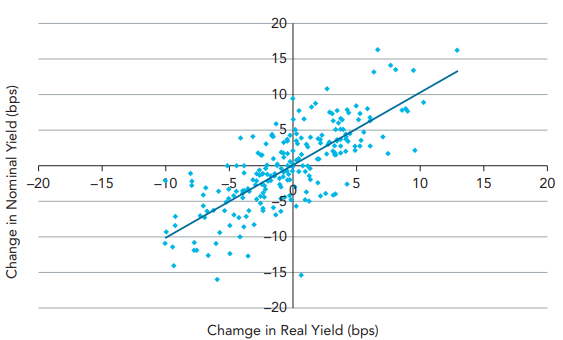
\includegraphics[width=0.70\linewidth]{fig/p111-004.png}
\end{center}
\figcap{Daily changes in yield of the two bonds from 17 August 2009 to 2 July 2010. The cloud
slopes upward at slightly more than 45 degrees, which is the whole justification for the beta
adjustment that follows. The R-squared is around 80\%.}

% ---------------------------------------------------------
\lo{MR-11 c}{Calculate the regression hedge adjustment factor, beta.}

In order to profit from a hedge, we must assume \term{variability in the spread} between the
real and nominal yields over time. Least squares regression is conducted to analyse these
changes. The alpha and beta coefficients of a least squares regression line are determined by
the line of best fit through historical yield data points.

\begin{mrfmlbox}
\[ \Delta y_t^{\,N} \;=\; \alpha + \beta\, \Delta y_t^{\,R} + \epsilon_t \]
\mrvk{$\Delta y_t^{\,N}$ = changes in the \textit{nominal} yield (the dependent variable);\quad
$\Delta y_t^{\,R}$ = changes in the \textit{real} yield (the independent variable);\quad
$\alpha$ = the intercept;\quad $\beta$ = the slope, i.e.\ the hedge adjustment factor;\quad
$\epsilon_t$ = the error term.}{}
\end{mrfmlbox}

If least squares estimation determines the yield beta to be \term{1.0198}, this means that over
the sample period the nominal yield increases by 1.0198 basis points for every basis point
increase in real yields.

\begin{mrfmlbox}
\[ F^R \;=\; F^N \times \left( \frac{DV01^N}{DV01^R} \right) \times \beta \]
\mrvk{the same DV01 ratio as before, now scaled by the yield beta. A $\beta$ above 1 means the
nominal yield moves more than the real yield, so \textit{more} of the real bond is needed.}{}
\end{mrfmlbox}

% ---------------------------------------------------------
\lo{MR-11 d}{Calculate the face value of an offsetting position needed to carry out a regression hedge.}

Defining $F^R$ and $F^N$ as the face amounts of the real and nominal bonds respectively, and
their corresponding DV01s as $DV01^R$ and $DV01^N$, the DV01 hedge is adjusted by the hedge
adjustment factor beta.

\begin{center}
\begin{tikzpicture}[every node/.style={font=\scriptsize\sffamily},
  stepb/.style={rectangle, rounded corners=3pt, line width=0.8pt,
    text width=3.0cm, align=center, inner sep=6pt, minimum height=1.35cm}]
  \node[stepb, draw=black!45, fill=FRMSoft] (a) at (0,0)
    {\textbf{\$100M}\\ T-bond sold\\ \textit{$F^N$}};
  \node[stepb, draw=FRMNavy!60, fill=PaleNavy] (b) at (4.6,0)
    {\textbf{\$80.95M}\\ DV01-neutral hedge};
  \node[stepb, draw=FRMGreen!60, fill=PaleGreen] (c) at (9.2,0)
    {\textbf{\$82.55M}\\ regression hedge};
  \draw[FRMGold, -{Stealth[length=5pt]}, line width=1pt] (a) -- (b)
    node[midway, above, text=black, align=center]
    {$\times \dfrac{0.068}{0.084}$};
  \draw[FRMGold, -{Stealth[length=5pt]}, line width=1pt] (b) -- (c)
    node[midway, above, text=black, align=center]
    {$\times\ \beta = 1.0198$};
  \node[anchor=north, text=black!60, align=center, text width=3.2cm] at (4.6,-0.85)
    {corrects for \textbf{size}};
  \node[anchor=north, text=black!60, align=center, text width=3.6cm] at (9.2,-0.85)
    {corrects for \textbf{yield sensitivity}};
\end{tikzpicture}
\end{center}
\figcap{Two separate corrections, applied in sequence. The DV01 ratio scales for the size of the
underlying instrument; beta then scales for the fact that nominal and real yields do not move
one-for-one.}

This regression hedge approach suggests that for every \$100 million sold in T-bonds, we should
buy \term{\$82.55 million} in TIPS. This accounts for hedging not only the size of the
underlying instrument, but also differences between nominal and real yields over time.

The example showed that the beta coefficient in the regression hedge was close to one, meaning
the hedge closely resembled the DV01-neutral hedge. However, it is important to acknowledge that
the assumption of a \term{constant beta coefficient} may not always be valid.

\begin{mrkeybox}[title={Other factors to consider}]
\begin{itemize}
\item \term{R-squared}, which indicates the percentage of variation in nominal yields explained
      by changes in real yields.
\item The \term{standard error of the regression (SER)}, which measures the standard deviation
      of the actual error terms in the regression model.
\end{itemize}
\medskip
Higher R-squared and lower SER values suggest a stronger relationship and a better fit of the
regression model, respectively.
\end{mrkeybox}

% ---------------------------------------------------------
\lo{MR-11 e}{Calculate the face value of multiple offsetting swap positions needed to carry out a two-variable regression hedge.}

Regression hedging can also be conducted with \term{two} independent variables. For example, a
trader in euro interest rate swaps buys/receives the fixed rate in a relatively illiquid 20-year
swap and wishes to hedge this interest rate exposure. Since it may be impractical to hedge this
position by immediately selling 20-year swaps, the trader may choose to sell a combination of
10- and 30-year swaps.

\begin{mrfmlbox}
\[ \Delta y_t^{\,20} \;=\; \alpha + \beta^{10}\, \Delta y_t^{\,10}
   + \beta^{30}\, \Delta y_t^{\,30} + \epsilon_t \]
\mrvk{$\Delta y_t^{\,20}$ = change in the 20-year swap rate, the position being hedged;\quad
$\beta^{10}$, $\beta^{30}$ = the two risk weights, which are what the face values are built
from.}{}
\end{mrfmlbox}

The beta coefficients in the regression model represent \term{risk weights}, which are used to
calculate the face value of multiple offsetting positions:

\begin{mrfmlbox}
\[ \frac{-\bigl(F^{10} \times DV01^{10}\bigr)}{F^{20} \times DV01^{20}} \;=\; \beta^{10}
   \qquad\qquad
   \frac{-\bigl(F^{30} \times DV01^{30}\bigr)}{F^{20} \times DV01^{20}} \;=\; \beta^{30} \]
\vspace{-8pt}
\[ F^{10} \;=\; -\,\frac{F^{20} \times DV01^{20}}{DV01^{10}} \times \beta^{10}
   \qquad\qquad
   F^{30} \;=\; -\,\frac{F^{20} \times DV01^{20}}{DV01^{30}} \times \beta^{30} \]
\mrvk{the minus sign carries the \textit{short} position: the hedge legs are sold against the long
20-year swap. Each face value divides by \textit{its own} DV01, not the 20-year DV01.}{}
\end{mrfmlbox}

\begin{mrexbox}[title={Example --- two-variable regression output}]
The trader runs an initial regression using data on changes in the 10-, 20-, and 30-year euro
swap rates for a five-year period.
\end{mrexbox}

\begin{center}
\small
\begin{tabular}{l r r}
\arrayrulecolor{FRMRule}\toprule
\rowcolor{FRMNavy} \hdr{} & \hdr{Value} & \hdr{Standard error}\\
Number of observations & 1,281 & \\
\rowcolor{FRMSoft} R-squared & 99.8\% & \\
Standard error & 0.14 & \\
\midrule
\rowcolor{FRMSoft} Alpha & $-0.0014$ & 0.0040\\
Change in 10-year swap rate & 0.2221 & 0.0034\\
\rowcolor{FRMSoft} Change in 30-year swap rate & 0.7765 & 0.0037\\
\bottomrule
\end{tabular}
\end{center}

\begin{center}
\begin{tikzpicture}[every node/.style={font=\scriptsize\sffamily}]
  \fill[PaleNavy, draw=FRMNavy!60, line width=0.7pt] (0,0) rectangle (2.664,0.8);
  \fill[PaleGreen, draw=FRMGreen!60, line width=0.7pt] (2.664,0) rectangle (11.982,0.8);
  \draw[black!40, dashed, line width=0.7pt] (12.0,-0.25) -- (12.0,1.15);
  \node[text=FRMNavy] at (1.33,0.4) {\textbf{10-year: 22.21\%}};
  \node[text=FRMGreen] at (7.32,0.4) {\textbf{30-year: 77.65\%}};
  \node[anchor=south, text=black!55] at (12.0,1.17) {100\%};
  \node[anchor=north, text=black!60] at (6.0,-0.28)
    {the two weights sum to 99.86\%, so the hedge DV01 is very close to the 20-year swap DV01};
\end{tikzpicture}
\end{center}
\figcap{The trader hedges 22.21\% of the 20-year swap DV01 with a 10-year swap and 77.65\% with
a 30-year swap. Because the weights sum to approximately one, the regression hedge DV01 lands
very close to the 20-year swap DV01 --- but it is the regression, not an assumption, that puts
them there.}

\begin{mrkeybox}
The two-variable approach will provide a better hedge, in terms of R-squared, compared to a
single-variable approach. However, regression hedging is \term{not an exact science}.
\end{mrkeybox}

% ---------------------------------------------------------
\lo{MR-11 f}{Compare and contrast level and change regressions.}

In regression-based hedges there are two main approaches. Both estimate regression coefficients
to establish a relationship between two bond yields, but they differ in how they handle the
data.

\begin{center}
\small
\begin{tabularx}{\linewidth}{@{}p{3.5cm} p{4.4cm} >{\raggedright\arraybackslash}X@{}}
\arrayrulecolor{FRMRule}\toprule
\rowcolor{FRMNavy} \hdr{Approach} & \hdr{Equation} & \hdr{What is regressed on what}\\
\textbf{1. Change-on-change}
  & $\Delta y_t = \alpha + \beta\,\Delta x_t + \Delta \epsilon_t$\newline
    where $\Delta y_t = y_t - y_{t-1}$\newline and $\Delta x_t = x_t - x_{t-1}$
  & \textit{Changes} in yields are regressed on \textit{changes} in yields.\\
\rowcolor{FRMSoft}
\textbf{2. Level-on-level}
  & $y_t = \alpha + \beta x_t + \epsilon_t$
  & Bond \textit{yields} are regressed on bond \textit{yields}, without considering the changes.\\
\textbf{3. Autoregressive model}
  & $\epsilon_t = \rho\,\epsilon_{t-1} + v_t$
  & Assumes today's error term is composed of some part of yesterday's error term plus a new
    random fluctuation $v_t$.\\
\bottomrule
\end{tabularx}
\end{center}

\begin{mrkeybox}[title={Note --- true in both change and level regressions}]
\begin{itemize}
\item The estimated regression coefficients $\alpha$ and $\beta$ are \term{unbiased and
      consistent}.
\item The error terms $\epsilon_t$ are \term{likely to be correlated over time}.
\end{itemize}
\end{mrkeybox}

% ---------------------------------------------------------
\lo{MR-11 g}{Explain why and how a regression hedge differs from a hedge based on a reverse regression.}

\noindent\gapbadge\hspace{4pt}{\sffamily\fontsize{7.6}{9}\selectfont\color{black!55}%
This objective does not appear in either layer of the source notes. It is written below from the
GARP curriculum so the objective is not left blank.}\par
\vspace{6pt}

\begin{mrgapbox}[title={What the objective asks for}]
Given a regression of $y$ on $x$, another trader could instead regress $x$ on $y$. The two
regressions produce \textit{different} slope coefficients, and therefore different hedges for
what looks like the same trade. The objective is to explain why the two differ, and why neither
is simply wrong.
\end{mrgapbox}

\subsection{The setup}
Consider hedging a corporate bond position with a Treasury bond. The \term{original regression}
regresses daily changes in the corporate bond's yield on daily changes in the Treasury's yield.
The \term{reverse regression} does the opposite, regressing the Treasury's yield changes on the
corporate's.

\begin{center}
\small
\begin{tabular}{l r r}
\arrayrulecolor{FRMRule}\toprule
\rowcolor{FRMNavy} \hdr{} & \hdr{Regression} & \hdr{Reverse regression}\\
$\beta$ & 0.842 & 0.921\\
\rowcolor{FRMSoft} Standard error & 2.00 & 2.09\\
\midrule
Implied risk weight & 84.2\% & $1/0.921 = $ \textbf{108.6\%}\\
\bottomrule
\end{tabular}
\end{center}
\figcap{The same two bonds, the same data window, two regressions --- and two risk weights that
are not remotely the same. Note that the reverse regression's implied weight is the
\textit{reciprocal} of its beta, not the beta itself.}

\begin{mrkeybox}[title={Why the two differ}]
\begin{enumerate}
\item \term{Least squares is not symmetric.} Regressing $y$ on $x$ minimises the squared errors
      measured \textit{vertically}; regressing $x$ on $y$ minimises them \textit{horizontally}.
      These are different minimisation problems, so they produce different lines and therefore
      different slopes. The two betas coincide only if the fit is perfect.
\item \term{They answer different questions.} Each regression minimises the variance of a hedge
      of a \textit{particular} position. The original regression minimises the variance of
      hedging a chosen face amount of the corporate bond; the reverse regression minimises the
      variance of hedging a chosen face amount of the Treasury.
\item \term{The two trades are not comparable.} Because each fixes a different leg, the two
      hedged positions carry different volatilities. They are different trades, not two answers
      to the same question.
\end{enumerate}
\end{mrkeybox}

\begin{mrtrapbox}[title={The point to state out loud}]
Neither hedge is ``right'' and the other ``wrong''. The choice of \textit{which} position to fix
is what defines the trade. A regression hedge minimises the variance of hedging the face amount
the trader actually committed to. Trades with other objectives --- holding a fixed amount of the
hedging instrument, or targeting a fixed amount of volatility risk --- are constructed
differently.
\end{mrtrapbox}

% ---------------------------------------------------------
\lo{MR-11 h}{Describe principal component analysis and explain how it is applied to constructing a hedging portfolio.}

Regression analysis hedging looks at specific bond yields and their pairwise correlations.
\term{Principal component analysis} provides a broader and more general description of how the
\textit{entire term structure} behaves, by identifying a smaller set of uncorrelated factors
that can explain the movement of interest rates across all bonds.

For example, consider a set of swap rates with maturities ranging from 1 to 30 years. PCA
identifies a small number of uncorrelated factors that effectively capture the risks across all
the interest rates. It may create 30 factors, each representing a change in one of the 30 rates,
but these factors are chosen in a way that captures the most important information about the
entire term structure.

\begin{mrkeybox}[title={Properties of PCA}]
\begin{enumerate}
\item The sum of the variances of the 30 principal components equals the sum of the variances of
      the individual rates. The PCs thus \term{capture the volatility} of the set of rates.
\item The PCs are \term{not correlated} with each other.
\item Each PC is chosen to contain the \term{highest possible variance}, given the earlier PCs.
\end{enumerate}
\end{mrkeybox}

The advantage of this approach is that we only really need to describe the volatility and
structure of the \term{first three} PCs, since the sum of the variances of the first three PCs
is a good approximation of the sum of the variances of all rates.

\begin{center}
\begin{tikzpicture}
\begin{axis}[
  width=11.0cm, height=6.3cm,
  xmin=0, xmax=31, ymin=-1.6, ymax=4.2,
  xlabel={\scriptsize Term (years)},
  ylabel={\scriptsize Basis points per one standard deviation move},
  xlabel style={font=\scriptsize}, ylabel style={font=\scriptsize},
  tick label style={font=\scriptsize},
  xtick={1,5,10,15,20,25,30}, ytick={-1,0,1,2,3,4},
  legend style={font=\scriptsize\sffamily, draw=FRMRule, fill=white,
    at={(0.5,-0.30)}, anchor=north, legend columns=-1, column sep=10pt},
  axis line style={draw=black!55}, clip=false]
\addplot[black!35, line width=0.6pt, forget plot, domain=0:31, samples=2] {0};
\addplot[FRMNavy, line width=1.2pt, mark=*, mark size=1.1pt] coordinates {
(1,0.23)(2,0.59)(3,1.18)(4,1.77)(5,2.28)(6,2.64)(7,2.94)(8,3.14)(9,3.31)
(10,3.44)(15,3.65)(20,3.73)(30,3.77)};
\addlegendentry{PC1 --- ``level''}
\addplot[FRMRed, line width=1.2pt, dashed, mark=*, mark size=1.1pt] coordinates {
(1,-0.16)(2,-0.51)(3,-0.99)(4,-1.16)(5,-1.12)(6,-0.89)(7,-0.60)(8,-0.36)(9,-0.13)
(10,0.07)(15,0.71)(20,1.02)(30,1.35)};
\addlegendentry{PC2 --- ``slope''}
\addplot[FRMGreen, line width=1.2pt, dotted, mark=*, mark size=1.1pt] coordinates {
(1,0.29)(2,0.47)(3,0.42)(4,0.23)(5,0.02)(6,-0.13)(7,-0.20)(8,-0.24)(9,-0.25)
(10,-0.23)(15,0.00)(20,0.17)(30,0.36)};
\addlegendentry{PC3 --- ``short rate'' / curvature}
\end{axis}
\end{tikzpicture}
\end{center}
\figcap{The first three principal components of USD LIBOR swap rates, from the GARP curriculum's
worked data set. PC1 moves every rate the same direction and is roughly flat beyond seven years,
hence ``level''. PC2 pushes short rates down while long rates rise, hence ``slope''. PC3 is
small and changes sign twice across the curve, hence ``curvature''. This figure is not in the
source notes; it is added because the objective asks you to \textit{describe} PCA, and the
shapes are what there is to describe.}

\begin{mrkeybox}[title={Benefits of PCA hedging}, breakable=false]
\begin{itemize}
\item \term{Reduces complexity:} describe the curve with just three factors, capturing most of
      the variance, instead of a full covariance matrix.
\item \term{Easier to manage:} analyse and hedge based on three factors instead of many
      individual rates.
\end{itemize}
\end{mrkeybox}


% ==========================================================
